\documentclass{article}

% TEMP PACKAGES!
\usepackage[utf8]{inputenc}
\usepackage[russian]{babel}
\usepackage{amsmath}
\usepackage{cmap}

% These ones should be added to the article's .tex file...
\usepackage{tikz}
\usepackage{pgfplots}
\usepackage{verbatim}
\usepackage{standalone}
\usepackage{array}
\usepackage{amsmath,amssymb}

\usepackage{url}

%... and these rows too.
\pgfplotsset{ every non boxed x axis/.append style={x axis line style=-},
     every non boxed y axis/.append style={y axis line style=-}}
\pgfplotsset{compat = 1.3}
\newcolumntype{P}[1]{>{\centering\arraybackslash}p{#1}}

\renewcommand{\vec}[1]{{\boldsymbol #1}}

\begin{document}

\section{Сравнение BigARTM с другими библиотеками}

Сравниваем BigARTM с реализацией алгоритма Online VB LDA в библиотеке для тематического моделирования Gensim\footnote{\url{http://radimrehurek.com/gensim/}} и Vowpal Wabbit\footnote{\url{https://github.com/JohnLangford/vowpal_wabbit/wiki/Latent-Dirichlet-Allocation}}. Для сравнения будем строить тематическую модель для документов из английской Википедии (корпус описан далее). 

\paragraph{Перплексия.} Алгоритм LDA представляет тематическую модель в виде распределений Дирихле на строчки $\Theta$ и столбцы $\Phi$:
\begin{gather}
	\vec{\theta}_{d} \sim \text{Dir}(\vec{\gamma}_d), \quad \vec{\phi}_{t} \sim \text{Dir}(\vec{\lambda}_t)
\end{gather}
Для того чтобы сравнить перплексию матриц $\Phi, \Theta$ для hold-out документов, мы будем брать средние распределения 
\begin{gather}
	\vec{\theta}^\text{mean}_d = \mathbb{E}_{\text{Dir}(\vec{\gamma}_d)}\vec{\theta}_d, \quad \vec{\phi}^\text{mean}_t = \mathbb{E}_{\text{Dir}(\vec{\gamma}_d)} \vec{\phi}_t.
\end{gather}
 
\paragraph{Параметры эксперимента}
\begin{itemize}
	\item Машина: x86\_64, 32 ядра, 1324.898MHz
	\item Corpus: English Wikipedia shapshot \texttt{2014-12-08}, hold-out 100'000 documents
	\item Topics: 100
	\item One pass through train documents of the corpus
	\item Batch size: 10'000 (\texttt{chunksize} in Gensim, \texttt{--minibatch} in VW)
	\item Update rule: $\rho = (\tau_0 + t)^{-\kappa}$, $\tau_0 = 1$, $\kappa = 0.5$
	\item Update after each batch in non-parallel implementation, update after $P$ batches when running in $P$ parallel threads (\texttt{update\_every = num\_processors})
	\item LDA Priors: $\alpha = 0.1,\, \beta = 0.1$ ($\vec{\theta}_d \sim \text{Dir}(\alpha),\, \vec{\phi}_t \sim \text{Dir}(\beta)$)
\end{itemize}


\begin{table}
	\centering
	\label{tab:libraries_comparison}

	\begin{tabular}[t]{c|c|ccc}
	\hline
	Library & Proc. & Train Time & Inference Time & Perplexity \\
	\hline
	BigARTM Smoothing & 1 & 62 min & 127 sec & 4000 \\
	Gensim LDA & 1 & 369 min & 395 sec & 4161 \\
	Vowpal Wabbit LDA & 1 & 73 min & 120 sec & 4108 \\
	\hline
	BigARTM Smoothing & 8 & 8 min & 24 sec & 4304 \\
	Gensim LDA-Multicore & 8 & 70 min & 338 sec & 4470 \\
	\end{tabular}
	\caption{Сравнение BigARTM с реализацией LDA в библиотеке Gensim и Vowpal Wabbit. Train Time — время на обучение модели, Inference Time — время вычисления $\theta_d$ для всех документов из hold-out. Perplexity — перплексия посчитанная по обученной модели $\{\vec{\phi}_t\}$ на hold-out документах $\{vec{\theta}_d\}$, в случае Gensim и VW в качестве распределений $\vec{\phi}_t$ и $\vec{\theta}_d$ брались средние из соответствующих распределений Дирихле.}
\end{table}

\begin{figure}
	\centering
	\label{fig:bigartm_speedup}
	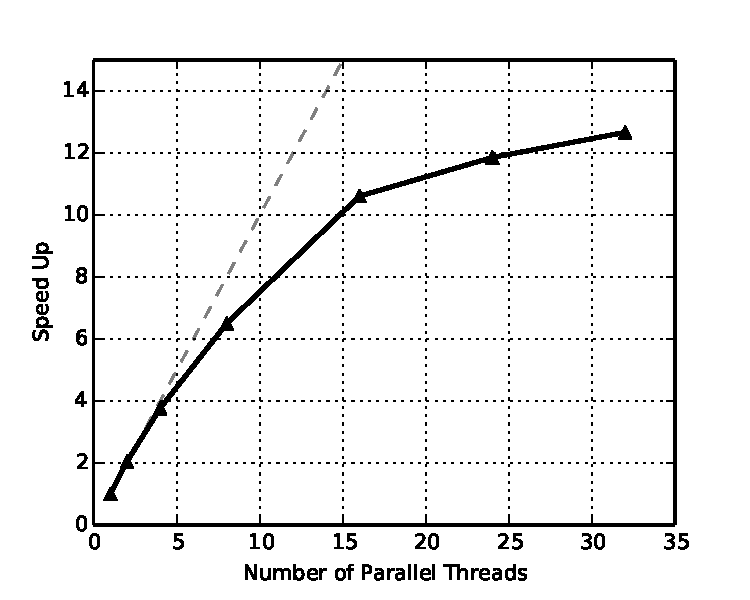
\includegraphics[height=6cm]{bigartm_speedup}
	\caption{BigARTM speed up }
\end{figure}



\section{On LDA and ARTM}

Данный раздел посвящён сравнению моделей LDA и ARTM. В экспериментах, сравнивающих BigARTM с Gensim и VW.LDA, мы показали, что алгоритм Online PLSA со сглаживающим регуляризатором и Online VB LDA работают схожим образом. Поэтому в этом эксперименте будут оцениваться характеристики PLSA со сглаживающим регуляризатором (который мы далее будем называть LDA) и ARTM (суть PLSA с набором регуляризаторов).

\paragraph{Текстовая коллекция} Все наши эксперименты проводились на корпусе английской Википедии
\footnote{Коллекция была получена с помощью gensim.make\_wikicorpus.}
, объём которой $|D| \approx 3.7 \times 10^6$ документов. Словарь имеет размер $|W| \approx 10^5$, общая длина коллекции в словах $n \approx 577 \times 10^6$.

\paragraph{Параметры эксперимента}
В этом эксперименте мы будем пользоваться следующими функционалами качества моделирования:
\begin{itemize}
	\item Перплексия на контрольной выборке\
	\footnote{Объём контрольной выборки, на которой перплексия измерялась в ходе прохода по коллекции --- 10 тыс. документов. Кроме того, была измерена результирующая перплексия на выборке из 100 тыс. документов.}.
	\item Разреженность матрицы $\Phi$.
	\item Разреженность матрицы $\Theta$ документов обучающей выборки.
	\item Характеристики ядер тем (размер, чистота, контрастность) (\cite{LABEL} ССЫЛКА НА НУЖНУЮ ПУБЛИКАЦИЮ КВ!!!).
\end{itemize}
Обе модели будут иметь следующий общий набор параметров, с которыми будет запускаться BigARTM: 1 проход по коллекции
\footnote{Подразумевается один полный проход по всей коллекции и повторный проход по первым $1.5 \times 10^5$ документам для уточнения их распределений.}
, 10 проходов по каждому документу, 100 выделяемых тем. Матрица $\Theta$, построенная на предыдущем проходе по документу, используется в качестве начального приближения на текущем. Параметры обновления матрицы $\Phi$, $\kappa$ и $\tau_0$, равны 0.5 и 64 соответственно
\footnote{Как это было в экспериментах в \ref{LABEL} РАЗДЕЛ ПРО СРАВНЕНИЕ БИБЛИОТЕК!!!}
. Порог $p(t|w)$ для ядровых функционалов --- 0.25,. Размер батча равен 10000, обновления модели производится каждые батч.

Параметры LDA $\alpha = \beta = \cfrac{1}{|T|}$.

\begin{figure}[h!]
\begin{tabular}{cc}
\documentclass{standalone}

\usepackage{tikz}
\usepackage{pgfplots}
\usepackage{verbatim}

\pgfplotsset{ every non boxed x axis/.append style={x axis line style=-},
     every non boxed y axis/.append style={y axis line style=-}}     
\pgfplotsset{compat = 1.9}

\begin{document}
\scriptsize

\begin{tikzpicture}[remember picture, baseline=0pt, scale = 0.8]
    \begin{axis}[
        ylabel shift = -3 pt,
        width=7cm,
        height=5cm,
        axis lines=left,
        ymajorgrids=true,
        xmajorgrids=true,
        ymin = 0, ymax = 100000,
        major grid style={draw=lightgray},
        ylabel={\scriptsize $\mathrm{\bf Perplexity}$},
        scaled x ticks = false,                    
        ]
    \addplot[smooth,line width=0.4mm] plot coordinates {
		(80000, 93308)
		(210000, 69748)
		(350000, 40293)
		(470000, 33250)
		(600000, 24970)
		(750000, 20488)
		(860000, 17735)
		(1020000, 15461)
		(1130000, 14215)
		(1250000, 12848)
		(1390000, 11726)
		(1500000, 11023)
		(1640000, 10443)
		(1750000, 10016)
		(1870000, 9555)
		(2000000, 9128)
		(2130000, 8829)
		(2260000, 8527)
		(2360000, 8300)
		(2480000, 8071)
		(2630000, 7858)
		(2740000, 7713)
		(2860000, 7511)
		(2990000, 7345)
		(3100000, 7227)
		(3260000, 7084)
		(3360000, 6996)
		(3508494, 6889)
		(3658494, 6781)
		(3718494, 6723)
    }; \label{perplexityPlsa}
    
    \addplot[smooth,line width=0.2mm] plot coordinates {
		(80000, 93470)
		(210000, 85201)
		(340000, 52457)
		(470000, 35692)
		(600000, 27265)
		(750000, 21531)
		(860000, 19200)
		(1020000, 16156)
		(1130000, 14820)
		(1250000, 13445)
		(1390000, 12148)
		(1500000, 11393)
		(1640000, 10815)
		(1760000, 10255)
		(1870000, 9812)
		(2010000, 9290)
		(2140000, 8958)
		(2250000, 8663)
		(2350000, 8418)
		(2480000, 8149)
		(2620000, 7908)
		(2730000, 7750)
		(2850000, 7536)
		(2990000, 7303)
		(3100000, 7178)
		(3260000, 7016)
		(3360000, 6926)
		(3518494, 6786)
		(3658494, 6670)
		(3718494, 6623)    
    }; \label{perplexityLda}
    \end{axis}
    
    \begin{axis}[
    	ylabel shift = -7 pt,
        width=7cm,
        height=5cm,
        axis lines=left,
        axis x line*=top,
        xtick=\empty,
        axis y line*=right,
        ymin = 0, ymax = 100,
        ylabel near ticks,             
        ylabel={\scriptsize $\mathrm{\bf Sparsity}$},
        legend columns=3, 
        legend style={
            text width=5.5em,
            text height=1.5ex,
            text depth=.5ex,        
        	draw=none,
            /tikz/column 3/.style={
                column sep=0pt,
            },
            at={(axis description cs:1.14,-0.14)}
        },
        every axis legend/.append style={nodes={right}},
        ]
    \addlegendimage{black}        
    \addlegendimage{dashed, black} 
    \addlegendimage{dotted, black}
    \addlegendimage{/pgfplots/refstyle=perplexityPlsa}\addlegendentry{\scriptsize $\mathrm{\:\; Perplexity}$} 
    \addplot[dashed,line width=0.4mm] plot coordinates {
		(80000, 2)
		(210000, 71)
		(350000, 67)
		(470000, 68)
		(600000, 72)
		(750000, 75)
		(860000, 78)
		(1020000, 80)
		(1130000, 82)
		(1250000, 83)
		(1390000, 84)
		(1500000, 85)
		(1640000, 89)
		(1750000, 90)
		(1870000, 90)
		(2000000, 91)
		(2130000, 91)
		(2260000, 92)
		(2360000, 92)
		(2480000, 93)
		(2630000, 93)
		(2740000, 93)
		(2860000, 93)
		(2990000, 94)
		(3100000, 94)
		(3260000, 94)
		(3360000, 94)
		(3508494, 94)
		(3658494, 94)
		(3718494, 95)
    };           
    \addlegendentry{\scriptsize $\mathrm{\hphantom{A}\hphantom{A}Phi}$}

    \addplot[dashed,line width=0.2mm] plot coordinates {
		(80000, 2)
		(210000, 0)
		(340000, 0)
		(470000, 0)
		(600000, 0)
		(750000, 0)
		(860000, 0)
		(1020000, 0)
		(1130000, 0)
		(1250000, 0)
		(1390000, 0)
		(1500000, 0)
		(1640000, 0)
		(1760000, 0)
		(1870000, 0)
		(2010000, 0)
		(2140000, 0)
		(2250000, 0)
		(2350000, 0)
		(2480000, 0)
		(2620000, 0)
		(2730000, 0)
		(2850000, 0)
		(2990000, 0)
		(3100000, 0)
		(3260000, 0)
		(3360000, 0)
		(3518494, 0)
		(3658494, 0)
		(3718494, 0)
    };
    
    \addplot[dotted,line width=0.4mm] plot coordinates {
		(80000, 0)
		(210000, 0)
		(350000, 3)
		(470000, 25)
		(600000, 42)
		(750000, 52)
		(860000, 58)
		(1020000, 63)
		(1130000, 66)
		(1250000, 69)
		(1390000, 71)
		(1500000, 73)
		(1640000, 75)
		(1750000, 76)
		(1870000, 77)
		(2000000, 78)
		(2130000, 79)
		(2260000, 80)
		(2360000, 80)
		(2480000, 81)
		(2630000, 82)
		(2740000, 82)
		(2860000, 83)
		(2990000, 83)
		(3100000, 83)
		(3260000, 84)
		(3360000, 84)
		(3508494, 84)
		(3658494, 85)
		(3718494, 85)
    };         
    \addlegendentry{\scriptsize $\mathrm{\hphantom{A}\hphantom{A}Theta}$}  
    
    \addplot[dotted,line width=0.2mm] plot coordinates {
		(80000, 0.000000)
		(210000, 0.000000)
		(340000, 0.010000)
		(470000, 0.010000)
		(600000, 0.030000)
		(750000, 0.140000)
		(860000, 0.340000)
		(1020000, 0.700000)
		(1130000, 0.880000)
		(1250000, 0.800000)
		(1390000, 0.720000)
		(1500000, 0.650000)
		(1640000, 0.610000)
		(1760000, 0.560000)
		(1870000, 0.530000)
		(2010000, 0.490000)
		(2140000, 0.460000)
		(2250000, 0.440000)
		(2350000, 0.420000)
		(2480000, 0.400000)
		(2620000, 0.380000)
		(2730000, 0.360000)
		(2850000, 0.350000)
		(2990000, 0.330000)
		(3100000, 0.320000)
		(3260000, 0.300000)
		(3360000, 0.290000)
		(3518494, 0.280000)
		(3658494, 0.270000)
		(3718494, 0.270000)	
    };
    \end{axis}
\end{tikzpicture}
\normalsize

\end{document}
&
\documentclass{standalone}

\usepackage{tikz}
\usepackage{pgfplots}
\usepackage{verbatim}

\pgfplotsset{ every non boxed x axis/.append style={x axis line style=-},
     every non boxed y axis/.append style={y axis line style=-}}     
\pgfplotsset{compat = 1.3}

\begin{document}
\scriptsize

\begin{tikzpicture}[remember picture, baseline=0pt, scale = 0.8]
    \begin{axis}[
        ylabel shift = -2 pt,
        width=7cm,
        height=5cm,
        axis lines=left,
        ytick = {0, 200, 400, 600, 800, 1000},
        ymajorgrids=true,
        xmajorgrids=true,        
		scaled y ticks = true,
		scaled y ticks=base 10:-3,
        ymin = 0, ymax = 1100,
        major grid style={draw=lightgray},
        ylabel={\scriptsize $\mathrm{\bf Kernel~size}$},
        scaled x ticks = false,                   
        ]
    \addplot[smooth,line width=0.4mm] plot coordinates {
		(80000, 7)
		(210000, 471)
		(350000, 635)
		(470000, 741)
		(600000, 873)
		(750000, 957)
		(860000, 1000)
		(1020000, 1029)
		(1130000, 1044)
		(1250000, 1055)
		(1390000, 1062)
		(1500000, 1066)
		(1640000, 1064)
		(1750000, 1066)
		(1870000, 1065)
		(2000000, 1062)
		(2130000, 1057)
		(2260000, 1054)
		(2360000, 1049)
		(2480000, 1046)
		(2630000, 1042)
		(2740000, 1038)
		(2860000, 1036)
		(2990000, 1032)
		(3100000, 1030)
		(3260000, 1026)
		(3360000, 1023)
		(3508494, 1020)
		(3658494, 1017)
		(3718494, 1014)
    }; \label{kernelSizePlsa}
    
    \addplot[smooth,line width=0.2mm] plot coordinates {
		(80000, 7)
		(210000, 4)
		(340000, 20)
		(470000, 67)
		(600000, 162)
		(750000, 335)
		(860000, 433)
		(1020000, 480)
		(1130000, 539)
		(1250000, 615)
		(1390000, 679)
		(1500000, 717)
		(1640000, 745)
		(1760000, 775)
		(1870000, 790)
		(2010000, 824)
		(2140000, 837)
		(2250000, 859)
		(2350000, 867)
		(2480000, 880)
		(2620000, 894)
		(2730000, 895)
		(2850000, 903)
		(2990000, 920)
		(3100000, 927)
		(3260000, 936)
		(3360000, 937)
		(3518494, 945)
		(3658494, 954)
		(3718494, 952)    
    }; \label{kernelSizeLda}
    \end{axis}
    
    \begin{axis}[
    	ylabel shift = -4 pt,
        width=7cm,
        height=5cm,
        axis lines=left,
        axis x line*=top,
        xtick=\empty,
        axis y line*=right,
        ymin = 0, ymax = 1.1,
        ylabel near ticks,             
        ylabel={\scriptsize $\mathrm{\bf Purity~and~contrast}$},
        legend columns=3, 
        legend style={
            text width=4.5em,
            text height=1.5ex,
            text depth=.5ex,
        	draw=none,
            /tikz/column 3/.style={
                column sep=0pt,
            },
            at={(axis description cs:0.98,-0.14)}
        },        
        ]
    \addlegendimage{smooth, black}        
    \addlegendimage{dashed, black} 
    \addlegendimage{dotted, black}
    \addlegendimage{/pgfplots/refstyle=perplexityPlsa}\addlegendentry{\scriptsize $\mathrm{\hphantom{A}Size}$} 
    \addplot[dashed,line width=0.4mm] plot coordinates {
		(80000, 0.000000)
		(210000, 0.006000)
		(350000, 0.013000)
		(470000, 0.030000)
		(600000, 0.065000)
		(750000, 0.109000)
		(860000, 0.153000)
		(1020000, 0.199000)
		(1130000, 0.237000)
		(1250000, 0.266000)
		(1390000, 0.301000)
		(1500000, 0.331000)
		(1640000, 0.384000)
		(1750000, 0.402000)
		(1870000, 0.409000)
		(2000000, 0.427000)
		(2130000, 0.445000)
		(2260000, 0.455000)
		(2360000, 0.469000)
		(2480000, 0.481000)
		(2630000, 0.491000)
		(2740000, 0.503000)
		(2860000, 0.505000)
		(2990000, 0.513000)
		(3100000, 0.521000)
		(3260000, 0.527000)
		(3360000, 0.536000)
		(3508494, 0.542000)
		(3658494, 0.547000)
		(3718494, 0.553000)
    };           
    \addlegendentry{\scriptsize $\mathrm{\hphantom{A}Purity}$}

    \addplot[dashed,line width=0.2mm] plot coordinates {
		(80000, 0.000000)
		(210000, 0.001000)
		(340000, 0.002000)
		(470000, 0.010000)
		(600000, 0.023000)
		(750000, 0.051000)
		(860000, 0.073000)
		(1020000, 0.104000)
		(1130000, 0.125000)
		(1250000, 0.151000)
		(1390000, 0.177000)
		(1500000, 0.201000)
		(1640000, 0.220000)
		(1760000, 0.238000)
		(1870000, 0.250000)
		(2010000, 0.270000)
		(2140000, 0.287000)
		(2250000, 0.297000)
		(2350000, 0.309000)
		(2480000, 0.323000)
		(2620000, 0.335000)
		(2730000, 0.343000)
		(2850000, 0.354000)
		(2990000, 0.363000)
		(3100000, 0.369000)
		(3260000, 0.379000)
		(3360000, 0.384000)
		(3518494, 0.393000)
		(3658494, 0.400000)
		(3718494, 0.403000)
    };
    
    \addplot[dotted,line width=0.4mm] plot coordinates {
		(80000, 0.313000)
		(210000, 0.559000)
		(350000, 0.501000)
		(470000, 0.527000)
		(600000, 0.540000)
		(750000, 0.557000)
		(860000, 0.572000)
		(1020000, 0.585000)
		(1130000, 0.596000)
		(1250000, 0.605000)
		(1390000, 0.614000)
		(1500000, 0.622000)
		(1640000, 0.646000)
		(1750000, 0.651000)
		(1870000, 0.654000)
		(2000000, 0.660000)
		(2130000, 0.667000)
		(2260000, 0.671000)
		(2360000, 0.676000)
		(2480000, 0.680000)
		(2630000, 0.683000)
		(2740000, 0.687000)
		(2860000, 0.689000)
		(2990000, 0.691000)
		(3100000, 0.693000)
		(3260000, 0.696000)
		(3360000, 0.698000)
		(3508494, 0.700000)
		(3658494, 0.702000)
		(3718494, 0.704000)
    };         
    \addlegendentry{\scriptsize $\mathrm{\hphantom{A}Contrast}$}  
    
    \addplot[dotted,line width=0.2mm] plot coordinates {
		(80000, 0.308000)
		(210000, 0.303000)
		(340000, 0.328000)
		(470000, 0.337000)
		(600000, 0.350000)
		(750000, 0.373000)
		(860000, 0.386000)
		(1020000, 0.390000)
		(1130000, 0.400000)
		(1250000, 0.413000)
		(1390000, 0.427000)
		(1500000, 0.436000)
		(1640000, 0.443000)
		(1760000, 0.451000)
		(1870000, 0.456000)
		(2010000, 0.466000)
		(2140000, 0.471000)
		(2250000, 0.477000)
		(2350000, 0.480000)
		(2480000, 0.485000)
		(2620000, 0.489000)
		(2730000, 0.491000)
		(2850000, 0.494000)
		(2990000, 0.499000)
		(3100000, 0.502000)
		(3260000, 0.506000)
		(3360000, 0.507000)
		(3518494, 0.510000)
		(3658494, 0.513000)
		(3718494, 0.513000)	
    };
    \end{axis}
\end{tikzpicture}
\normalsize
\end{document}
\end{tabular}
\caption{Comparison of LDA (thin) and ARTM (bold) models. X axis is a number of processed documents.} \label{fig:comparison_plot}
\end{figure}

Регуляризатор для ARTM, представляющий собой смесь разреживания и декорреляции тем, описывается формулой

\begin{align}
    R(\Phi,\Theta)
    =&
    - \beta \sum_{t\in T} \sum_{w\in W} \beta_w \ln \phi_{wt}
    - \alpha \sum_{d\in D} \sum_{t\in T} \alpha_t \ln \theta_{td}
    \notag
\\  {}&
    - \gamma
        \sum_{t\in T}
        \sum_{s\in T\backslash t}
        \sum_{w\in W} \phi_{wt}\phi_{ws}
    \to \max.
\end{align}

Отсюда получаются формулы M-шага

\begin{align}
    \phi_{wt} &\propto
        \Bigl(n_{wt}
            - \beta \underbrace{\beta_{w} [t\!\in\! T]}_{\substack{\text{sparsing}\\\text{topic}}} {}
            - \gamma \underbrace{[t\!\in\! T]\: \phi_{wt} \!\sum_{s\in T\backslash t}\! \phi_{ws}}_{\text{decorrelation}} {}
        \Bigr)_{+};
\\
    \theta_{td} &\propto
        \Bigl(n_{td}
            - \alpha \underbrace{\alpha_{t} [t\!\in\! T]}_{\substack{\text{sparsing}\\\text{topic}}} {}
        \Bigr)_{+}.
\end{align}

Коэффициенты $\beta_w$ и $\alpha_t$ примем равными 1, $\forall w,t$. Коэффициенты регуляризации $\alpha,  \beta$ и $\gamma$ возьмём постоянными на протяжении всего прохода по коллекции. Их значения: $\alpha = 0.15, \beta = 0.009, \gamma = 7.8 \times 10^5$.

\paragraph{Результаты} В таблице \ref{tab:model_comparison} приведены финальные значения функционалов качества после одного прохода по коллекции для моделей LDA и ARTM. Видно, что комбинация регуляризаторов разреживания и декорреляции улучшает качество результирующей модели с небольшими потерями перплексии.

\begin{table}[t]
\caption{Comparison of LDA and ARTM models. Quality functionals: $\mathcal{P}_{10k}$ $\mathcal{P}_{100k}$ --- hold-out perplexity on 10.000 and 100.000 documents sets, $\mathcal{S}_{\Phi}$, $\mathcal{S}_{\Theta}$ --- sparsity of $\Phi$ and $\Theta$ matrices (in \%), $\mathcal{K}_{s}$, $\mathcal{K}_{p}$, $\mathcal{K}_{c}$ --- average topic kernel size, purity and contrast respectively.}
\label{tab:model_comparison}
\begin{center}
\renewcommand{\arraystretch}{1.5}
\begin{tabular}[t]{P{10.5em}|P{3.5em} P{3.5em} P{3.5em} P{3.5em} P{3.5em} P{3.5em} P{3.5em} }
\hline
Model/Functional & $\mathcal{P}_{10k}$ & $\mathcal{P}_{100k}$ &  $\mathcal{S}_{\Phi}$ & $\mathcal{S}_{\Theta}$ &  $\mathcal{K}_{s}$ & $\mathcal{K}_{p}$ &  $\mathcal{K}_{c}$ \\
\hline
LDA              & 3499 & 3827 & 0.0  & 0.0  & 931  & 0.535 & 0.516 \\
ARTM             & 3592 & 3944 & 96.3 & 80.5 & 1135 & 0.810 & 0.732 \\
\hline
\end{tabular}
\end{center}
\end{table}

Более подробно процесс обучения представлен на \ref{fig:comparison_plot}. На верхнем графике показано убывание перплексии и замеры разреженностей матриц $\Phi$ и $\Theta$. На нижнем --- усреднённые характеристики ядер тем. Видно, что LDA совершенно не способствует разреживанию и даёт менее чистые и контрастные ядра тем, чем ARTM.

\end{document}
